\documentclass{beamer}
\usepackage[utf8]{inputenc}
\usepackage{colortbl}
\usetheme{JuanLesPins}
\mode<presentation>
\useoutertheme{smoothtree}
\usecolortheme{whale}
\usecolortheme{orchid}
\useinnertheme[shadow=true]{rounded}
% profondeur table des matieres
\setcounter{tocdepth}{1}
\setbeamerfont{block title}{size={}}
\title{Projet Tuteuré \\Gestion centralisée de machines virtuelles}
\author{Augustin Bocca Julien Tournois\\Sébastien Michaux Mathieu Lamouroux}
\institute{IUT de Nancy Charlemagne}
%\addtobeamertemplate{footline}{\insertframenumber/\inserttotalframenumber}
\begin{document}

\AtBeginSubsection[]
{
  \begin{frame}<beamer>
    \frametitle{Plan}
    \tableofcontents[currentsection,currentsubsection,hideothersubsections]
  \end{frame}
}

\begin{frame}
  \titlepage
\end{frame}

\begin{frame}
    \frametitle{Plan}
    \tableofcontents
\end{frame}

%%%%%%%%%%%%%%%%%%%%%%%%%%%%%%%%%%%%%%%%%%%%%%%%%%%%%%%%%%%%
\section{Le contexte}
\subsection{Le projet}
\begin{frame}{Le projet tuteuré}
 %%%% trouver une boite
\begin{block}{Intitulé}
Mettre en place, évaluer et comparer différents outils de gestion centralisée de machines virtuelles.
\end{block}
\pause
\begin{block}{Résultats attendus}
  \begin{itemize}
    \item guide d'installation et d'utilisation synthétique
\pause
    \item scripts
\pause
    \item démos à grande échelle sur grid5000
\pause
    \item avis critique
   \end{itemize}
\end{block}
\end{frame}

\subsection{Grid5000}
\begin{frame}{La plateforme Grid5000}
%%%%%%%%% PHOTO
\begin{block}{Vue d'ensemble}
  \begin{itemize}
    \item Grille Informatique
\pause
    \item Dix sites en France
\pause
    \item Réliés par RENATER
\pause
    \item Objectif scientifique
  \end{itemize}
\end{block}
\end{frame}

\begin{frame}{Architecture type d'un site}
  \begin{center}
    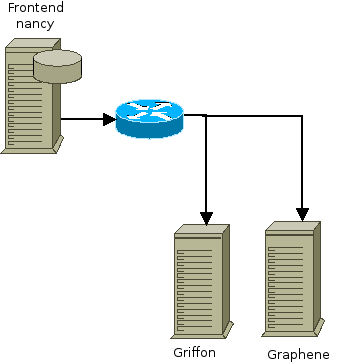
\includegraphics[width=180pt]{images_presentation/archi.png}
  \end{center}
\end{frame}

\begin{frame}{Connexion à un site}
  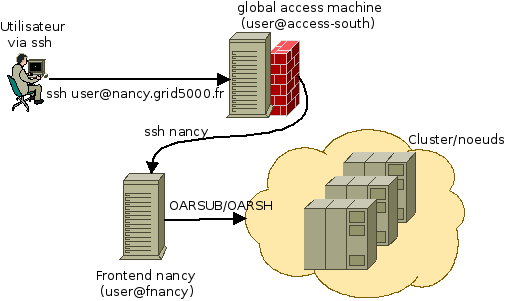
\includegraphics[width=330pt]{images_presentation/plan_site.png}
\end{frame}


%%%%%%%%%%%%%%%%%%%%%%%%%%%%%%%%%%%%%%%%%%%%%%%%%%%%%%%%%%%%
\section{La virtualisation}
\subsection{Historique}
\begin{frame}{Il était une fois la virtualisation...}
  \begin{description}
    \item[1960 : ] inventée par IBM pour optimiser l'utilisation du matériel sur les serveurs
\pause
    \item[1990 : ] VMware porte le concept sur les plateformes x86
\pause
    \item[Aujourd'hui : ] VMware se positionne en tant que leader du marché.
  \end{description}
\end{frame}

\subsection{Enjeux}
\begin{frame}{Pourquoi virtualisé?}
  Et c'est facile.
\end{frame}

%%%%%%%%%%%%%%%%%%%%%%%%%%%%%%%%%%%%%%%%%%%%%%%%%%%%%%%%%%%%
\section{Logiciels testés}
\subsection{Ganeti}
%%%%%%%% LOGO
\begin{frame}{Présentation}
  Et c'est facile.
\end{frame}
\begin{frame}{Installation}
  Et c'est facile.
\end{frame}
\begin{frame}{Utilisation}
  Et c'est facile.
\end{frame}
\begin{frame}{Démo}
  Et c'est facile.
\end{frame}

\subsection{Virt-Manager}
%%%%%%% LOGO
\begin{frame}{Présentation}
  Et c'est facile.
\end{frame}
\begin{frame}{Installation}
  Et c'est facile.
\end{frame}
\begin{frame}{Utilisation}
  Et c'est facile.
\end{frame}
\begin{frame}{Démo}
  Et c'est facile.
\end{frame}

%%%%%%%%%%%%%%%%%%%%%%%%%%%%%%%%%%%%%%%%%%%%%%%%%%%%%%%%%%%%
\section{Logiciels non-testés}

\subsection{Archipel}
%%%%% LOGO
\begin{frame}{Présentation}
  Et c'est facile.
\end{frame}
\begin{frame}{Installation}
  Et c'est facile.
\end{frame}
\begin{frame}{Utilisation}
  Et c'est facile.
\end{frame}

\subsection{OpenXenManager}
%%%%% LOGO
\begin{frame}{Présentation}
  Et c'est facile.
\end{frame}
\begin{frame}{Installation}
  Et c'est facile.
\end{frame}
\begin{frame}{Utilisation}
  Et c'est facile.
\end{frame}

%%%%%%%%%%%%%%%%%%%%%%%%%%%%%%%%%%%%%%%%%%%%%%%%%%%%%%%%%%%%
\section{Conclusion}
\subsection{Comparatif}
\begin{frame}{Comparaison des solutions testées}
\begin{center}
\begin{tabular}{|c|c|c|c|c|}
\hline
 & OXM & Ganeti & Virt-Manager & Archipel \tabularnewline
\hline
Documentation & 
\includegraphics[width=10pt]{images_presentation/bad.png} & 
\includegraphics[width=10pt]{images_presentation/ok.png} & 
\includegraphics[width=10pt]{images_presentation/moyen.png} & 
\includegraphics[width=10pt]{images_presentation/ok.png} \tabularnewline
\hline
Communauté &
\includegraphics[width=10pt]{images_presentation/moyen.png} & 
\includegraphics[width=10pt]{images_presentation/ok.png}& 
\includegraphics[width=10pt]{images_presentation/moyen.png}& 
\includegraphics[width=10pt]{images_presentation/moyen.png}\tabularnewline
\hline
Maturité &
\includegraphics[width=10pt]{images_presentation/moyen.png}  & 
\includegraphics[width=10pt]{images_presentation/ok.png} & 
\includegraphics[width=10pt]{images_presentation/ok.png}& 
\includegraphics[width=10pt]{images_presentation/moyen.png} \tabularnewline
\hline
Installation & 
\includegraphics[width=10pt]{images_presentation/moyen.png}&
\includegraphics[width=10pt]{images_presentation/moyen.png} & 
\includegraphics[width=10pt]{images_presentation/ok.png}& 
\includegraphics[width=10pt]{images_presentation/moyen.png}\tabularnewline
\hline
Réseau &
\includegraphics[width=10pt]{images_presentation/question.png}& 
\includegraphics[width=10pt]{images_presentation/moyen.png} & 
\includegraphics[width=10pt]{images_presentation/ok.png} & 
\includegraphics[width=10pt]{images_presentation/question.png}\tabularnewline
\hline
Sécurité & 
\includegraphics[width=10pt]{images_presentation/question.png}& 
\includegraphics[width=10pt]{images_presentation/ok.png} &
\includegraphics[width=10pt]{images_presentation/ok.png} & 
\includegraphics[width=10pt]{images_presentation/ok.png}
\includegraphics[width=10pt]{images_presentation/ok.png}\tabularnewline
\hline
Simplicité & 
\includegraphics[width=10pt]{images_presentation/ok.png}& 
\includegraphics[width=10pt]{images_presentation/moyen.png} & 
\includegraphics[width=10pt]{images_presentation/ok.png} & 
\includegraphics[width=10pt]{images_presentation/question.png}\tabularnewline
\hline
Flexibilité & 
\includegraphics[width=10pt]{images_presentation/question.png}& 
\includegraphics[width=10pt]{images_presentation/ok.png}& 
\includegraphics[width=10pt]{images_presentation/moyen.png}& 
\includegraphics[width=10pt]{images_presentation/question.png}\tabularnewline
\hline
\end{tabular}
\end{center}
\newline
*OXM : OpenXenManager
\end{frame}

%
\includegraphics[width=10pt]{images_presentation/moyen.png}
%
\includegraphics[width=10pt]{images_presentation/question.png}
%
\includegraphics[width=10pt]{images_presentation/bad.png}
%
\includegraphics[width=10pt]{images_presentation/ok.png}

\subsection{Problèmes rencontrés et bénéfices}
\begin{frame}{Problèmes rencontrés}
  Et c'est facile.
\end{frame}

\begin{frame}{Bénéfices}
  Et c'est facile.
\end{frame}

\end{document}
